%%%%%%%%%%%%%%%%%Epic 7, 8, 9, 10%%%%%%%%%%%%%%%%%%%%%%%%%%%%%%%%%%%%%%%%%%%%%%%%%%%%%%%

\subsection{Objekte erkennen}

Dieses Kapitel behandelt die Methoden zur Objekterkennung. Zur Identifikation der drei Klassen (Pylone, Knoten, Hindernisse) wurde das YOLOv11-Modell eingesetzt, das speziell für diese Aufgabe trainiert wurde. Ergänzend dazu dient ein Ultraschallsensor als Backup-System zur Erkennung von Hindernissen, um die Sicherheit des Roboters zu erhöhen. Die erzielten Modellresultate können anschließend vom Raspberry Pi ausgewertet werden damit der Roboter die optimale Route wählen kann.

Das finale Model wurde auf einem Datensatz Bilder trainiert welcher von der Raspberry-PI-Kamera aus der Betriebshöhe aufgenommen wurden. Der Datensatz enthält Bilder des Graphes, der Pylonen und der Hindernisse. 

\subsubsection{Kamera Halter}
\label{Kamera Halter}
Der Winkel und die Höhe der Kamera wurde in PREN1 an dem Testaufbau in Abb.\ref{fig:Testaufbau zum Festlegen des Kamerawinkels} getestet. Am Testaufbau konnte der Winkel zwischen der Kamera und der Vertikalen mit Hilfe einer Schraube verstellt werden. Der Winkel wurde so gewählt das er für die Bildverarbeitung ideal ist. 

Bei der Konstruktion der Kamerabefestigung wurde darauf geachtet, dass der Winkel wie im Testaufbau gemessen 23° Beträgt. Ebenfalls wichtig ist, dass die Linsen Höhe 242mm  über dem Boden beträgt. 


\begin{figure}[H]
\centering
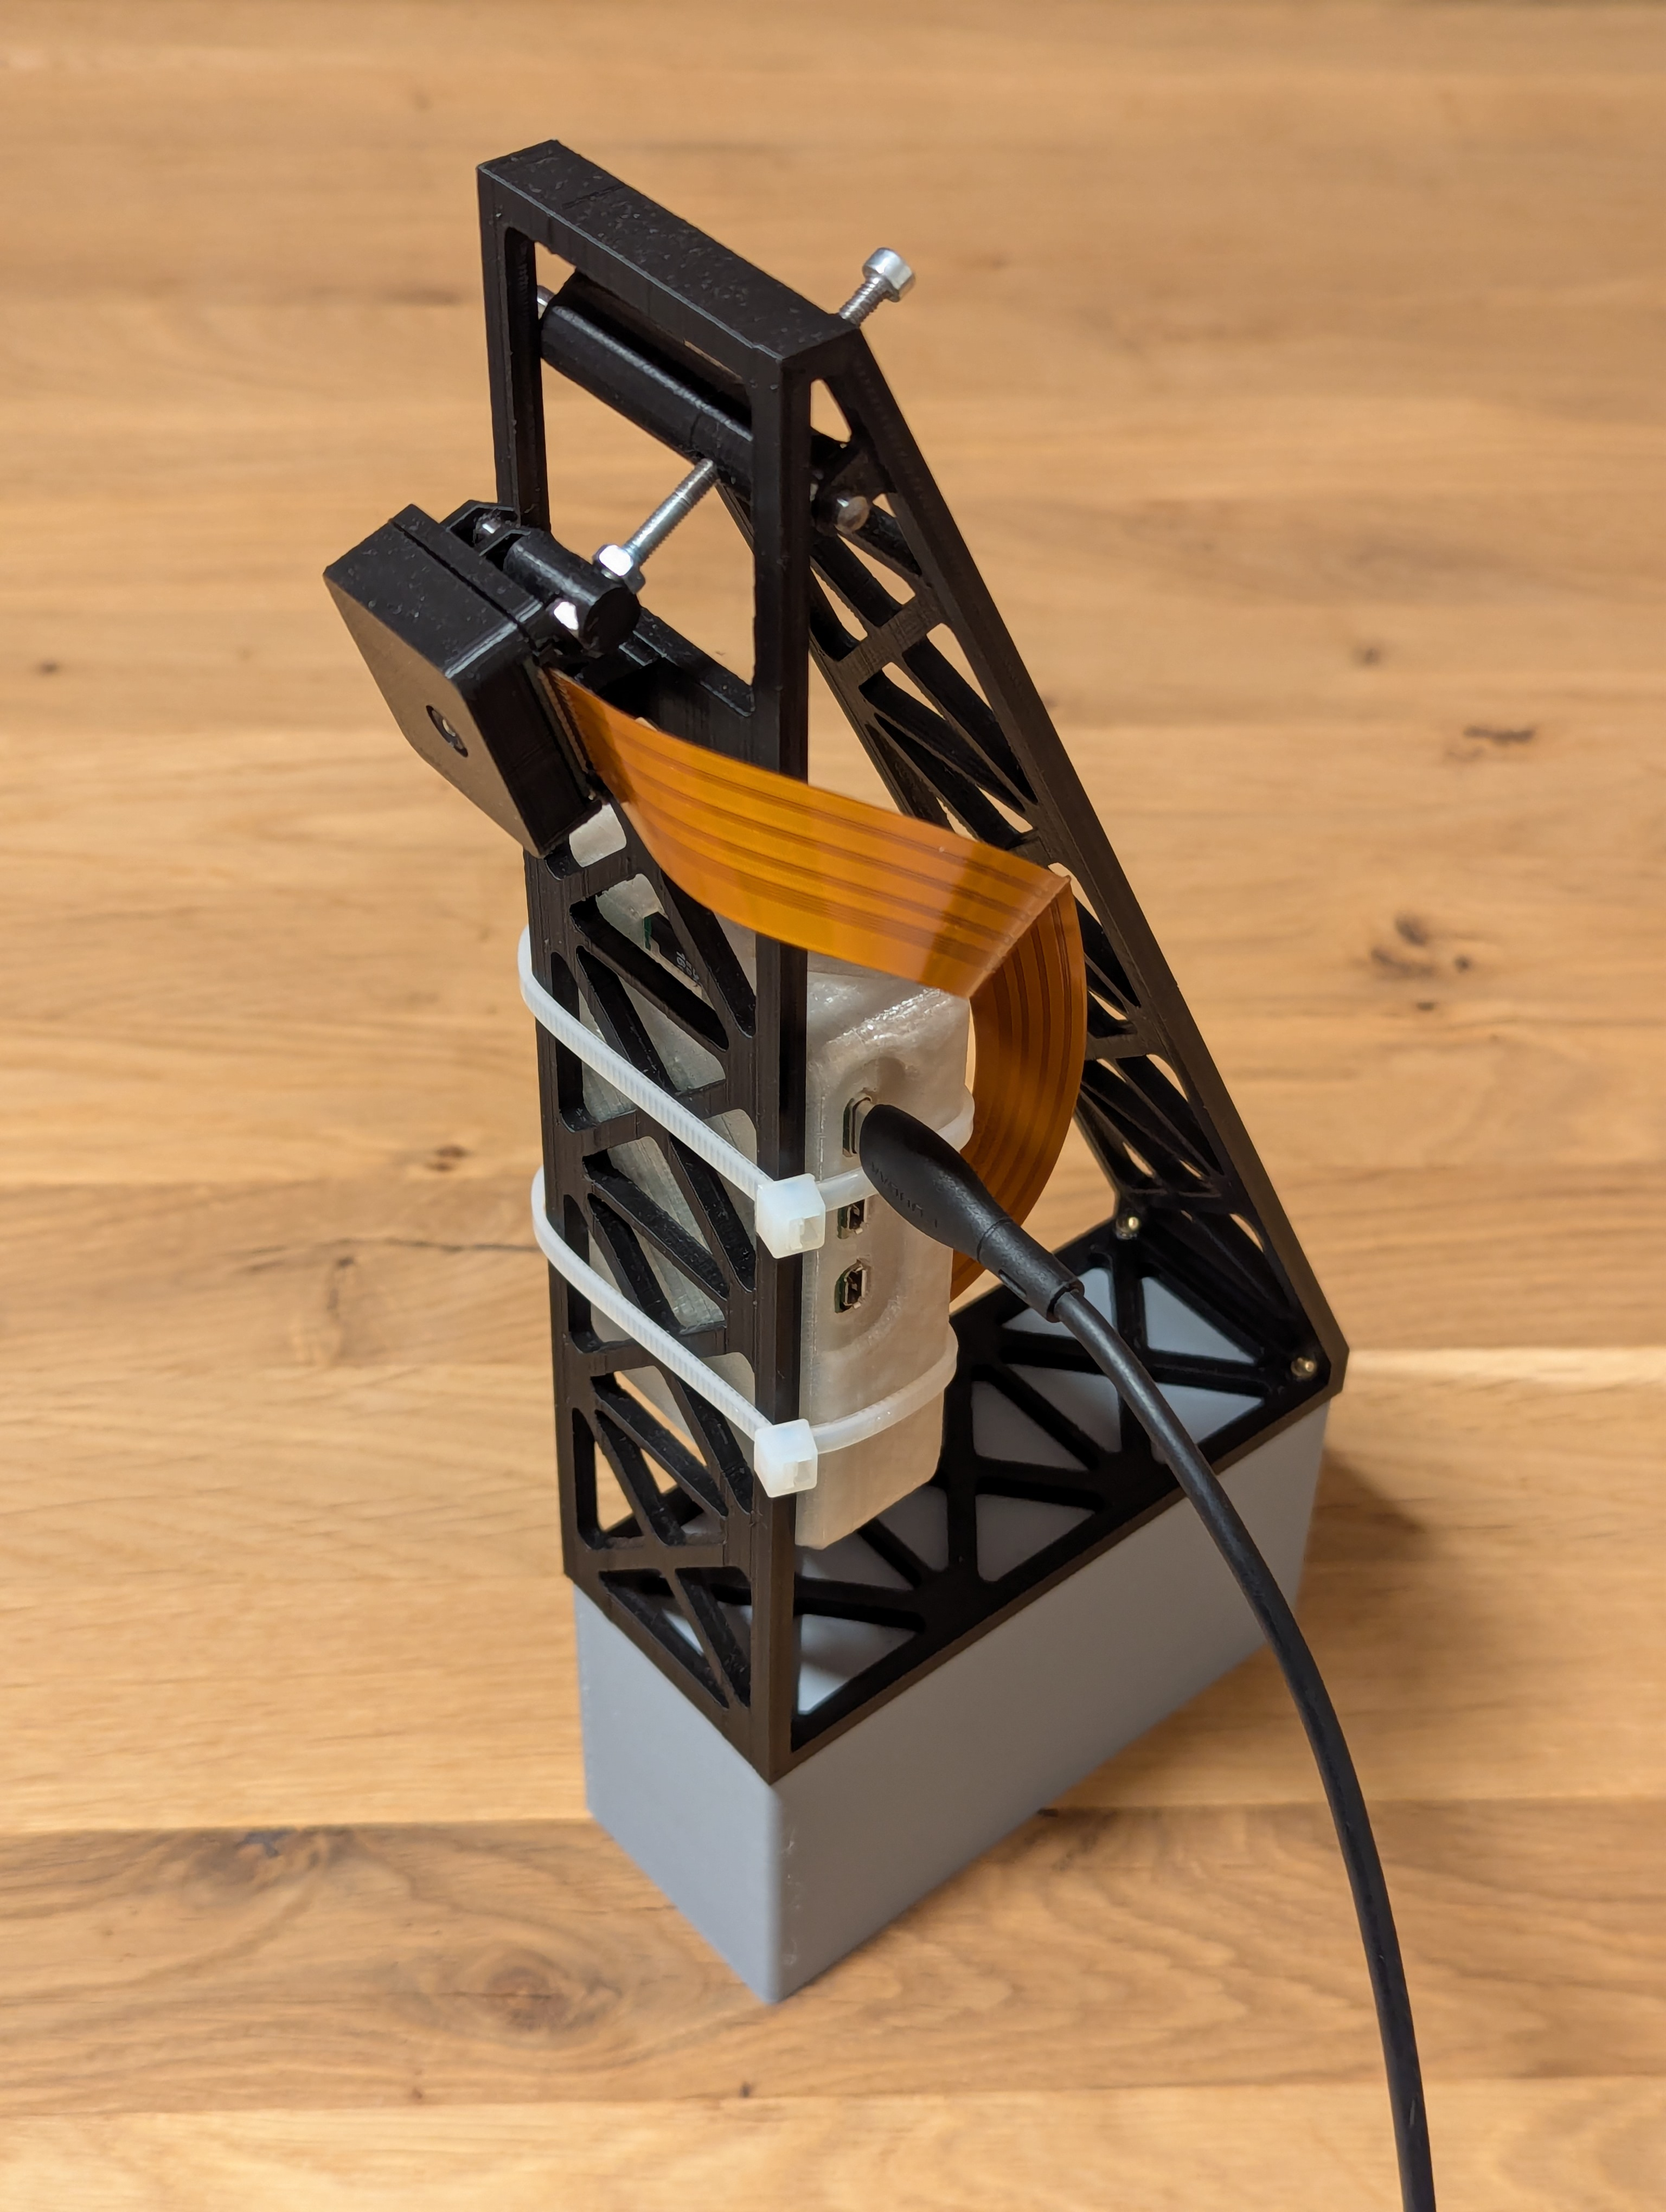
\includegraphics[width=5cm]{assets/MT/camer_tower_2.png}
\caption{Testaufbau zum Festlegen des Kamerawinkels}
\label{fig:Testaufbau zum Festlegen des Kamerawinkels}
\end{figure}

 \begin{figure}[H]
\centering
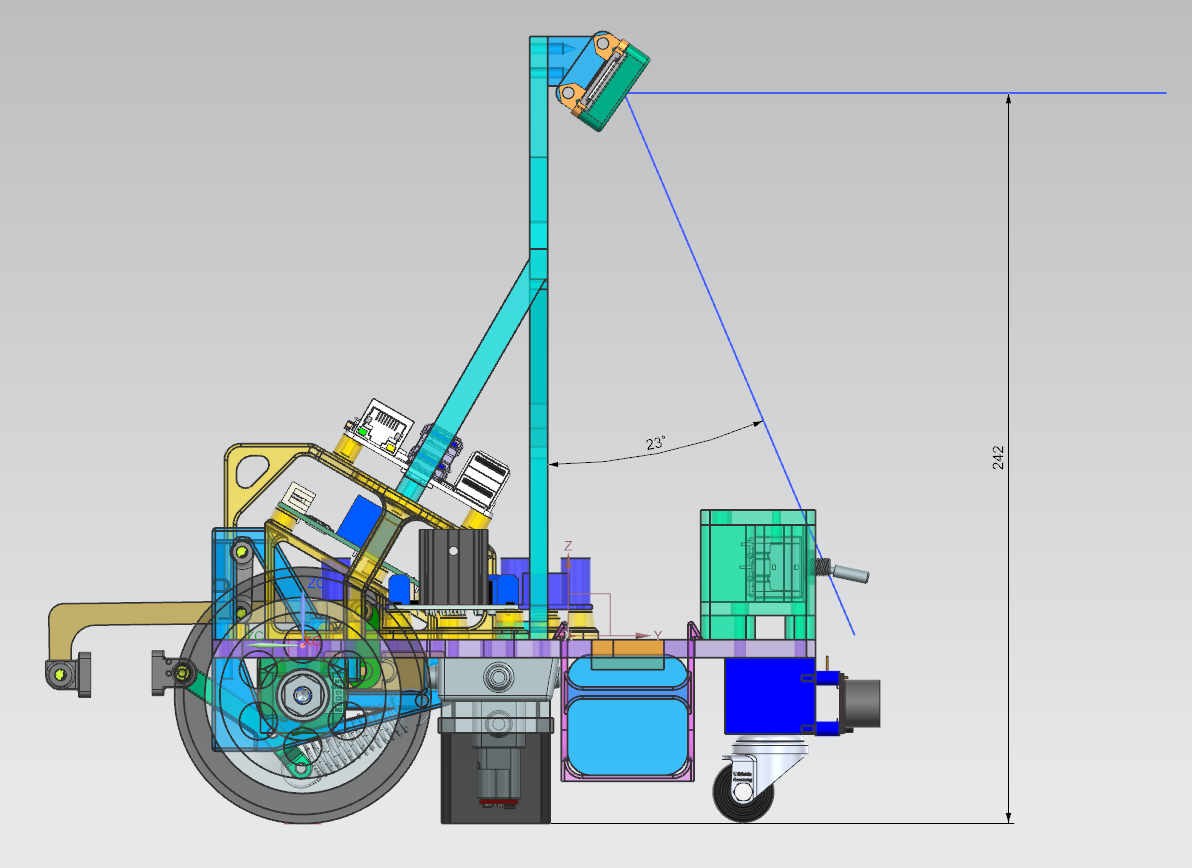
\includegraphics[width= \textwidth ]{assets/MT/Sichtfeld_Roboter.png}
\caption{Skizze der Funktionsmasse für die Kamerabefestigung}
\label{fig:Skizze der Funktionsmasse für die Kamerabefestigung}
\end{figure}


\subsubsection{Ultraschall}
\label{ultraschall}

Backup-Hinderniserkennung mittels Ultraschallsensor, um Risiko 12 (Objekte werden nicht erkannt) zu mitgieren.

Zur Erhöhung der Betriebssicherheit ist das Fahrzeug mit einer redundanten Hinderniserkennung ausgestattet. Diese erfolgt über einen Ultraschallsensor, der kontinuierlich die Entfernung zu Objekten im unmittelbaren Umfeld misst. Der Sensor ist direkt mit dem Mikrocontroller TinyK22 verbunden.

Die Messwerte werden in Echtzeit ausgewertet. Sobald ein Objekt in einer Distanz von weniger als 10 cm erkannt wird, wird automatisch ein Not-Stopp ausgelöst, um Kollisionen zu vermeiden. Gleichzeitig wird ein definierter Fehlercode generiert und über eine serielle Schnittstelle an den Raspberry Pi übertragen, um den Fehlerstatus zu protokollieren und entsprechende Massnahmen einleiten zu können.

\subsubsection{Training YOLOv11-Model trainieren}



Damit der Roboter Pylonen, Knoten und Hindernissen erkennen kann, wurde

Das Ziel war, das Modell auf einem Raspberry Pi 5 für den Einsatz in einem Roboter zu optimieren. Der Trainingsprozess umfasste drei Iterationen, wobei ich verschiedene Ansätze ausprobierte, um die Modellleistung zu verbessern. Diese Teil der Dokumentation beschreibt den Lernprozess, die Methodik, die Herausforderungen und die Ergebnisse der finalen Iteration.

Ein erfolgreich trainiertes Model hat die Fähigkeit zur Generalisierung. Das heisst, es ist besser Objekte zu erkennen in Bilder mit verschiedenen Bildkonditionen. Da das Datenset mit 116 Aufnahmen relativ klein ist, wurde künstliche Datenerweiterung angewendet. Durch "augmentation" werden die Bilder leicht in Helligkeit, Kontrast und weiteren Parametern verändert und diese den unveränderten Bildern hinzugefügt. So lernt das Model die selben Objekte in verschiedenen Konditionen zu erkennen.

Trainieren, auch Fine-Tuning genannt, eines YOLOv11-Modells ist „Supervised Learning“. Im Kontext von Computer Vision heisst das, jedes Bild wird mit Labels versehen, was in dem Bild zu sehen ist. Labeling, oder auch "annotation," wird mit dem Webtool Roboflow gemacht wo das annotierte Datenset im Yolov11-Format exportiert werden kann. 

Das eigentliche Training benötigt GPU-Rechenleistung. Mithilfe von Google Colab können kostenlos GPUs benutzt werden. Das Datenset wurde auf Google Colab hochgeladen und mit einem Jupiter Notebook dort trainiert.

\paragraph{Lernprozess und Trainingsiterationen}

\subparagraph{Erste Iteration}

In der ersten Iteration testete ich das YOLOv11n-Modell mit einem stark augmentierten Datensatz \text{(Rotation $\pm$30°, Helligkeit $\pm$50\%, Rauschen 10\%)}. Trainiert wurde mit einem Datensatz aus Bildern welche mit dem Mobiltelefon aufgenommen wurden. Zu Testzwecken hat dies ausgereicht. Für das Model welches dann eingesetzt wird, ist das suboptimal, da die Bilder mit denen trainiert wird, den Real-Konditionen entsprechen sollten.

Die Ergebnisse waren unbefriedigend, da die übermäßige Augmentation zu einem Überlernen (overfitting) künstlicher Muster führte, insbesondere bei der Klasse "Knoten." Darauf wurde mit Bildern der Raspberry Pi Kamera ein neuer Datensatz erstellt.


\subparagraph{Zweite Iteration: Iterative Erweiterung und Überanpassung}

In der zweiten Iteration kombinierte ich einen unveränderten Datensatz mit zwei erweiterten Datensätzen und trainierte iterativ mit je 300 Epochen.
Augmentationen umfassten horizontale Spiegelung, Rotation (±15°) und Helligkeit (

Diese Anzahl an Epochs war viel zu hoch was zu einem overfitting führte. Ausserdem erkannte ich Fehler in den Annotationen, die eine erneute Überarbeitung notwendig machten.

\subparagraph{Dritte Iteration: Kombination von Datensätzen und Finales Training}

In der dritten Iteration wurde der Ansatz optimiert, indem ein unveränderter Datensatz mit einem veränderten Datensatz kombiniert wurde, um Robustheit und Generalisierung zu verbessern.

Der unveränderte Datensatz umfasste 396 Bilder, annotiert in Roboflow. Der augmentierte Datensatz wurde gemäß Empfehlungen für den Einsatz im Innenraum mit variierenden Licht- und Bodenbedingungen erstellt. Die Augmentationseinstellungen waren:

\begin{itemize} 
    \item \textbf{Helligkeit}: $\pm$20\%, um Lichtvariationen abzubilden. 
    \item \textbf{Sättigung}: $\pm$10\%, für Farbänderungen. 
    \item \textbf{Farbton}: $\pm$5\%, für leichte Farbverschiebungen. 
    \item \textbf{Rauschen}: 5\% Gaussches Rauschen, für Sensorrauschen. 
    \item \textbf{Unschärfe}: 3-Pixel-Gaußsche Unschärfe, für Bewegungseffekte. 
\end{itemize}
Die Kombination der Datensätze erforderte ein zusammenfügen der Bilder in korrekter Ordnerstruktur und erfolgte in Google Colab per Kommandozeile.

Die Validierungs- und Testdaten stammten ausschließlich aus dem unveränderten Datensatz, um Datenlecks zu vermeiden. Die Konsistenz wurde durch Vergleich von Bild- und Label-Dateien überprüft.

Training und ErgebnisseDas Modell wurde mit folgendem Befehl trainiert:


\begin{verbatim}
yolo train model=yolo11n.pt data=/content/datasets/combined_dataset/data.yaml 
epochs=100 imgsz=640 batch=16 device=0 augment=True
\end{verbatim}

Die Validierungsergebnisse lauten:

\begin{itemize}
    \item \textbf{Model Architecture}: YOLOv11n (fused): 238 layers, 2,582,737 parameters, 0 gradients, 6.3 GFLOPs.
    \item \textbf{Overall Performance}:
    \begin{itemize}
        \item Images: 22
        \item Instances: 34
        \item Precision (P): 0.734
        \item Recall (R): 0.760
        \item mAP@0.5: 0.800
        \item mAP@0.5:0.95: 0.595
    \end{itemize}
    \item \textbf{Class Performance}:
    \begin{itemize}
        \item \textbf{Cone} (9 Images, 9 Instances):
        \begin{itemize}
            \item Precision: 0.796
            \item Recall: 1.0
            \item mAP@0.5: 0.955
            \item mAP@0.5:0.95: 0.824
        \end{itemize}
        \item \textbf{Node} (16 Images, 17 Instances):
        \begin{itemize}
            \item Precision: 0.759
            \item Recall: 0.529
            \item mAP@0.5: 0.611
            \item mAP@0.5:0.95: 0.299
        \end{itemize}
        \item \textbf{Obstacle} (8 Images, 8 Instances):
        \begin{itemize}
            \item Precision: 0.648
            \item Recall: 0.750
            \item mAP@0.5: 0.833
            \item mAP@0.5:0.95: 0.662
        \end{itemize}
    \end{itemize}
    \item \textbf{Speed} (per Image):
    \begin{itemize}
        \item Preprocess: 0.1 ms
        \item Inference: 1.7 ms
        \item Postprocess: 1.0 ms
        \item Total: ~2.8 ms (approx. 357 FPS on GPU)
    \end{itemize}
\end{itemize}


Die Ergebnisse zeigen eine starke Leistung bei "Kegel" und "Hindernis," während "Knoten" eine Schwäche darstellt, möglicherweise aufgrund unzureichender Daten oder Annotationen.

\paragraph{Reflexion des Lernprozesses}

Mein Lernprozess war iterativ geprägt. Die erste Iteration zeigte die Risiken von Überaugmentation, die zweite die Folgen von Überanpassung und fehlerhaften Annotationen. In der dritten Iteration integrierte ich diese Erkenntnisse, indem ich einen ausgewogenen Datensatz erstellte und die Epochenzahl optimierte. Google Colab und Roboflow waren entscheidend für den Erfolg.


\subsubsection{YOLOv11 Model konvertieren}
\label{convert-yolo}

Das .pt File des YOLO Models kann bereits eingelesen und verwendet werden. Es gibt Methoden, um diese Datei zu transformieren in ein anderes Format, damit auf embedded Systems und somit auch auf Raspberry Pis schneller die Bilderkennung durchgeführt werden kann.

Drei Möglichkeiten wurden betrachtet und verglichen:
TODO add sources for each \& akronyum
\begin{enumerate}
    \item Caffe2: In der Vergangenheit sehr geeignet, heutzutages mit PyTorch zusammengefügt und existiert nicht mehr auf diese Weise.
    \item NCNN: Sehr gute Performance für ARM Geräte (u.a. Raspberry Pi), sehr wenig Abhängigkeiten, einfache Transformation.
    \item ONXX: Geeignet für  Cross-Plattform Fälle, gute Austauschbarkeit des Models, flexibel, viele Abhängigkeiten.
\end{enumerate}

Es wird NCNN gewählt, da dies perfekt für den Use Case mit einem Raspberry Pi passt. Das erstellt .pt File kann mit der ultralytics Bibliothek transformiert werden:

\begin{verbatim}
yolo export model=best.pt format=ncnn
\end{verbatim}

Das Resultat ist ein Ordner mit zwei Dateien drin, mit allen nötigen Informationen, aus dem .pt File. Dieser Ordner kann im Python Code geladen werden, um die Bilderkennung durchzuführen. Mit der Transformation wurde das Risiko 3: 4 Minuten reichen nicht für einen Durchgang, weiter gemindert.

TODO: ADD NUMBERS, BEFORE (~1s) vs AFTER

\subsubsection{Modelresultate auswerten}
\label{model-results}

Um die Modelresultate auszuwerten wurde das Model in den Ordner der Navigation kopiert und es wurde eine ObjectDetector Klasse und ein Object Enum erstellt.

TODO UML

Diese ObjectDetector Klasse erstellt das Model aufgrund des NCNN Ordners bei der Instanzierung eines Objektes. Diese Objekt wird aufgerufen, wenn ein Nachbarsknoten geprüft werden soll und führt einen Prozess von drei Schritten durch:

\begin{enumerate}
    \item Inference (Objekterkennung)
    \item Resultat parsen
    \item Nächstes Objekte vor dem Roboter finden.
\end{enumerate}

Im Teil der Inference wird ein Bild an das Model gegeben. Dabei sollen nur die erkannten Objekte zurückgegeben werden, die mit einer definierten prozentualen Gewissheit erkannt wurden. Diese Gewissheit ist als Konstante definiert auf TODO WERT \& WIESO. \& falls Risiko damit vermindert (Falls erhoeht), Risiko 7

Diese Resultate werden dann geparsed, sodass alle erkannten Objekte mir ihrer ID, mit der Confidence, mit der sie erkannt wurden, und mit ihrem Standort auf dem Bild zurückgegeben werden.

Aus dieser Liste werden nun alle Objekte betrachtet, die sich auf der Mittellinie des Bildes befinden. Somit kann sichergestellt werden, dass nicht aus Versehen Objekte, die sich nicht auf der Fahrbahn, die betrachtet wird, befinden gespeichert werden und auch Risiko 7 (Objekte werden fälschlicherweise erkannt) kann so mitigiert werden. Die Mitellinie wird berechnet aus der Breite des Bildes. Diese Objekte werden sortiert nach ihren Koordinaten auf dem Bild. Das erste Element in dieser List, ist das nächste Objekt zum Roboter. Die Id des Objektes, die vom Model zurückgegben wird, korrespondiert mit der ID des erstellten Enums, damit das erkannte Objekt als Enum zurückgegeben wird.

In folgenden Fällen wird nicht einfach das nächste Objekt zurückgegeben:

\begin{itemize}
    \item Falls das nächste Objekt eine Barriere und das zweitnächste eine Pylone ist. In diesem Fall wird zurückgegeben, dass eine Pylone das nächste Objekt ist, da dieser Knoten sowieso nicht befahrbar ist und aus dem internen Graph entfernt werden soll.
    \item Falls kein Objekt erkannt wurde, wird ein Knoten zurückgegeben. Es ist weniger wahrscheinlich, dass eine Barriere oder ein Pylon verpasst werden, als dass ein Knoten nicht erkannt wird. Somit wird Risiko 2 (Knoten werden nicht erkannt) behandelt. Der Ultraschall kann trotzdem Objekte noch erkennen, falls ein unterwartetes Objekt auftritt. Es ist ein kleineres Problem ein Objekt zu verpassen, als sich eines einzubilden und fälschlicherweise Strecken zu entfernen. Durch den Ultraschall wird Risiko 12 und 1 (Objekte werden nicht erkannt) mitigiert.
\end{itemize}


Wie auf die einzelnen Objekte reagiert wird, ist in folgender Aufzählung beschrieben und ist gleich, wie in \acrshort{pren1} geplant.

\textbf{Pylonen erkennen}

Wird eine Pylone erkannt, wird der Knoten, der gerade geprüft wurde, inklusive alle Strecken dahin, aus dem internen Graphen entfernt.

\textbf{Knoten erkennen}

Wenn ein Knoten erkannt wird, dann geschieht nichts. Es wird interpretiert, dass sich kein Objekt auf diesem Weg befindet und die Strecke normal befahrbar ist.

\textbf{Barrieren erkennen}

Wir auf dem Bild eine Barriere erkannt, wird dies im internen Graphen gespeichert, indem die jeweilige Linie höher gewichtet wird, da es länger dauern wird diese zu überqueren.

\textbf{Entfernte Linien erkennen}

TODO LUKAS

\newpage
%%%%%%%%%%%%%%%%%Epic 11%%%%%%%%%%%%%%%%%%%%%%%%%%%%%%%%%%%%%%%%%%%%%%%%%%%%%%%
\subsection{Zieleingabe}

\subsubsection{Peripherie}
\label{zieleingabe}

Geht sehr schnell: 1 Minute aufstellen gemindert Risiko